% ****** Start of file apssamp.tex ******
%
%   This file is part of the APS files in the REVTeX 4.2 distribution.
%   Version 4.2a of REVTeX, December 2014
%
%   Copyright (c) 2014 The American Physical Society.
%
%   See the REVTeX 4 README file for restrictions and more information.
%
% TeX'ing this file requires that you have AMS-LaTeX 2.0 installed
% as well as the rest of the prerequisites for REVTeX 4.2
%
% See the REVTeX 4 README file
% It also requires running BibTeX. The commands are as follows:
%
%  1)  latex apssamp.tex
%  2)  bibtex apssamp
%  3)  latex apssamp.tex
%  4)  latex apssamp.tex
%
\documentclass[%
 reprint,
%superscriptaddress,
%groupedaddress,
%unsortedaddress,
%runinaddress,
%frontmatterverbose, 
%preprint,
%preprintnumbers,
%nofootinbib,
%nobibnotes,
%bibnotes,
 amsmath,amssymb,
 aps,
 %prl,
%pra,
%prb,
%rmp,
%prstab,
%prstper,
%floatfix,
]{revtex4-2}

\usepackage{graphicx}% Include figure files
\usepackage{dcolumn}% Align table columns on decimal point
\usepackage{bm}% bold math
%\usepackage{hyperref}% add hypertext capabilities
%\usepackage[mathlines]{lineno}% Enable numbering of text and display math
%\linenumbers\relax % Commence numbering lines

%\usepackage[showframe,%Uncomment any one of the following lines to test 
%%scale=0.7, marginratio={1:1, 2:3}, ignoreall,% default settings
%%text={7in,10in},centering,
%%margin=1.5in,
%%total={6.5in,8.75in}, top=1.2in, left=0.9in, includefoot,
%%height=10in,a5paper,hmargin={3cm,0.8in},
%]{geometry}
\usepackage{xcolor}
\usepackage{amsfonts}
\usepackage{amsmath}
\usepackage{amssymb}
\usepackage{braket}
\usepackage{url}
\usepackage{tocloft}
\renewcommand{\cftsecleader}{\cftdotfill{\cftdotsep}}
\usepackage[colorlinks=true,linkcolor=blue,citecolor=blue,urlcolor=blue]{hyperref}
\begin{document}
\bibliographystyle{plain}
\preprint{APS/123-QED}

\title{Generating function approach for precise coincidence detection of TMSV}% Force line breaks with \\

\author{Nico Sieber}

\date{\today}
\begin{abstract}
In this paper, we present a generating function approach to derive an analytical expression for the detection probabilities of a two-mode squeezed vacuum (TMSV) state transformed by a half-wave plate, using bucket detectors. Due to the lack of photon number resolution in bucket detectors, previous discussions on coincidence probabilities relied on approximations that considered only the first few terms of the TMSV state. In contrast, this work provides a complete derivation of the coincidence probabilities, accounting for all terms of the TMSV state generated by type II spontaneous parametric down-conversion (SPDC).
\end{abstract}
\maketitle
%\tableofcontents
\section{Generating and manipulating the two-mode squeezed vaccum}
We first have to discuss the underlying experimental scheme which is the basis of our presented work in this document. In figure \ref{fig:setup} we see that the state we will work with is generated by pumping a type II ppKTP crystal to generate degenerate photons. It has to be noted that a compensation crystal (same crystal without poling and half the length of the ppKTP crystal) has to be placed after the ppKTP crystal in order to compensate for the walkoff between the generated horizontal (H) and vertical (V) photons. The generated TMSV state is then sent through a half-wave plate (HWP) at an angle $\vartheta$. Before measuring the photons with a bucket detector, a polarizing beamsplitter (PBS) is used to spatially separate the H and V components of the state.
\begin{figure}[!h]
    \centering
    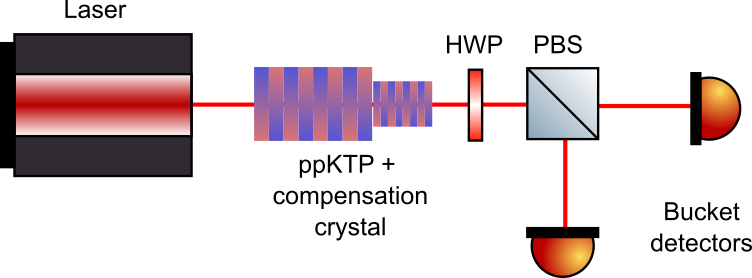
\includegraphics[width=\columnwidth]{experimentalSetupN00N.png}
    \caption{Schematic of the experimental setup discussed in this work.}
    \label{fig:setup}
\end{figure}
\section{\label{sec:s1} Simplified example}
Before we work on the full discussion involving the TMSV, we first show a simplified example of the calculation by only passing the state 
\begin{align}
\label{initial_state_simple}
    \ket{1_{H},1_{V}}=a_H^\dagger a_V^\dagger\ket{0,0}
\end{align}
through the HWP. In equation (\ref{initial_state_simple}), $a_{H,V}^\dagger$ are the bosonic creation operators (for $H$- and $V$-polarized light) following the relation

\begin{align}
\label{Fock}
    \ket{n}=\dfrac{1}{\sqrt{n!}}\left(a^\dagger\right)^n\ket{0}.
\end{align}

Assuming the fast axis of the HWP is aligned with the horizontal axis, the Jones matrix is given by

\begin{align}
\label{Jones}
    U_{\text{HWP}}(\vartheta) = 
    \begin{pmatrix}
    \cos(2\vartheta) & \sin(2\vartheta) \\
    \sin(2\vartheta) & -\cos(2\vartheta) 
    \end{pmatrix},
\end{align}

with $\vartheta$ being the angle of the HWP. With (\ref{initial_state_simple}) and (\ref{Jones}) we get the transformation

\begin{align}
\label{Tansformation:trafo}
    \begin{pmatrix}
    a_{H,\text{new}}^\dagger  \\
    a_{V,\text{new}}^\dagger
    \end{pmatrix}
    =
    \begin{pmatrix}
    \cos(2\vartheta) & \sin(2\vartheta) \\
    \sin(2\vartheta) & -\cos(2\vartheta) 
    \end{pmatrix}
    \cdot
    \begin{pmatrix}
    a_{H,\text{old}}^\dagger  \\
    a_{V,\text{old}}^\dagger
    \end{pmatrix},
\end{align}
which can be used to write the state after the HWP as
\begin{align}
\label{Transformation:state_simple}
    \ket{1_H,1_V}&=a_H^\dagger a_V^\dagger\ket{0,0}\notag\\
    &\overset{(\ref{Tansformation:trafo})}{\Rightarrow} \left(a_H^\dagger\cos(2\vartheta)+a_V^\dagger\sin(2\vartheta)\right)\notag\\
    &\times\left(a_H^\dagger\sin(2\vartheta)-a_V^\dagger\cos(2\vartheta)\right)\ket{0,0}.
\end{align}
Evaluating the terms of (\ref{Transformation:state_simple}) results in:
\begin{align}
    \cos(2\vartheta)\sin(2\vartheta)(a_H^\dagger)^2\ket{0,0} &= \sqrt{2}\cos(2\vartheta)\sin(2\vartheta)\ket{2,0} \label{Transformation:terms_simple1}\\
    -\cos(2\vartheta)\sin(2\vartheta)(a_H^\dagger)^2\ket{0,0} &= -\sqrt{2}\cos(2\vartheta)\sin(2\vartheta)\ket{0,2} \label{Transformation:terms_simple2}\\
    -\cos^2(2\vartheta)a_H^\dagger a_V^\dagger\ket{0,0} &= -\cos^2(2\vartheta)\ket{1,1} \label{Transformation:terms_simple3}\\
    \sin^2(2\vartheta)a_H^\dagger a_V^\dagger\ket{0,0} &= \sin^2(2\vartheta)\ket{1,1}\label{Transformation:terms_simple4}
\end{align}

Remark on notation: Equations (\ref{Transformation:terms_simple1})-(\ref{Transformation:terms_simple4}), the indices for polarization were left out and further wont be used anymore due to convenience. To further make it easier to differentiate which polarization is meant, the convention of choosing $H$ polarization for the first and $V$ polarization for the second mode when using the $\ket{\cdot}$-notation will strictly be followed (when using operator notation indices will be used).

Looking at the terms (\ref{Transformation:terms_simple1})-(\ref{Transformation:terms_simple4}), we see that for the $\vartheta=\pi/8+k\pi/4$ and $k=0,1,2,3,...$, the terms containing one $H$ and one $V$ photon cancel each other due to destructive interference. However, this case only happens under the following conditions:
\begin{itemize}
    \item[-] The $H$ and $V$ photons occupy the same spatial mode.
    \item[-] The photons must be indistinguishable in all degrees of freedom besides polarization.
\end{itemize}
Consequently, for $\vartheta=\pi/8$, the sum of terms (\ref{Transformation:terms_simple1})-(\ref{Transformation:terms_simple2}) becomes
\begin{align}
    \ket{1_H,1_V}&=a_H^\dagger a_V^\dagger\ket{0,0}\notag\\
    &\overset{(\ref{Tansformation:trafo}),\vartheta=\pi/8}{\Rightarrow}\dfrac{1}{\sqrt{2}}(\ket{2,0}-\ket{0,2}).
\end{align}
\section{\label{sec:s2} Discussion involving the Two-Mode Squeezed Vacuum}
The next step is to do the same steps which we did for the state in (\ref{initial_state_simple}) for the TSMV. In this section, we first will look at the mathematical formulation of the TMSV, how it behaves when transformed by the HWP, and how relevant detection probabilities can be derived.
\subsection{Mathematical description of the two-mode squeezed vacuum}
For the correct phase-matching conditions the previously mentioned conditions of spatial overlap and indistinguishability are met. Mathematically, the TMSV state can be expressed as
\begin{align}
\label{tmsv}
    \ket{\text{TMSV}}&=\sqrt{1-|\lambda|^2}\sum_{n=0}^{\infty}\lambda^n\ket{n,n}\\
                     &=\sqrt{1-|\lambda|^2}\sum_{n=0}^{\infty}\dfrac{\lambda^n}{n!}\left(a_H^\dagger\right)^n\left(a_V^\dagger\right)^n\ket{0,0},
\end{align}
with $n$ as the photon number and
\begin{align}
    \lambda=\tanh(r),
\end{align}
where $r$ is the squeezing parameter. 
\subsection{Transformation of the Two-Mode Squeezed Vacuum}
Sending the TMSV through a HWP results in
\begin{align}
\label{TMSV_HWP:full}
    \ket{\text{TMSV}_{\text{HWP}}}=\Lambda&\sum_{n=0}^{\infty}\dfrac{\lambda^n}{n!}\left(\cos(2\vartheta)a_H^\dagger+\sin(2\vartheta)a_V^\dagger\right)^n\notag\\ &\times\left(\sin(2\vartheta)a_H^\dagger-\cos(2\vartheta)a_V^\dagger\right)^n\ket{0,0},
\end{align}
where $\Lambda=\sqrt{1-|\lambda|^2}$ is used as an abbreviation. For $n=0$ we get
\begin{align}
    \sqrt{1-|\lambda|^2}\ket{0,0},
\end{align}
from which the probability of the no-click case can be derived:
\begin{align}
\label{Prob:no-click}
    P_{\text{no-click}}=\Lambda^2\braket{0,0|0,0}=1-|\lambda|^2.
\end{align}
Excluding the $n=0$ term from $\ket{\text{TMSV}_{\text{HWP}}}$ in (\ref{TMSV_HWP:full}) results in
\begin{align}
\label{TMSV_HWP:wo_vac}
    \ket{\Pi}=\Lambda&\sum_{n=1}^{\infty}\dfrac{\lambda^n}{n!}\left(\cos(2\vartheta)a_H^\dagger+\sin(2\vartheta)a_V^\dagger\right)^n\notag\\ &\times\left(\sin(2\vartheta)a_H^\dagger-\cos(2\vartheta)a_V^\dagger\right)^n\ket{0,0},
\end{align}
which is a non-normalized state. 
\subsection{Deriving the probabilities for one click and coincidences}
To derive the analytical expression for the coincidence probability it is easier to just derive the probability for the case in which only one bucket detector clicks ($P_{\text{1-click}}(\vartheta)$) and afterwards calculate the coincidence probability with the condition of
\begin{align}
\label{Prob:condition}
    1\overset{!}{=}P_{\text{no-click}}+P_{\text{1-click}}(\vartheta)+P_{\text{coinc.}}(\vartheta),
\end{align}
where $P_{\text{no-click}}$ is given in (\ref{Prob:no-click}) already. 
\subsubsection{Probability for one click}
As a start we omit all terms from the state given in (\ref{TMSV_HWP:wo_vac}) which would lead to coincidences, leaving us with
\begin{align}
\label{TMSV_HWP:wo_vac_wo_cc}
    \ket{\Phi}&=\Lambda\sum_{n=1}^{\infty}\dfrac{\lambda^n}{n!}\sin^n(2\vartheta)\cos^n(2\vartheta)\left(a_H^\dagger\right)^{2n}\ket{0,0}\notag\\
    &+\Lambda\sum_{n=1}^{\infty}\dfrac{\lambda^n}{n!}(-1)^n\sin^n(2\vartheta)\cos^n(2\vartheta)\left(a_V^\dagger\right)^{2n}\ket{0,0}.
\end{align}
Using (\ref{Fock}) and the trigonometric identity
\begin{align}
    \sin(x)\cos(x)=\dfrac{1}{2}\left(\sin(2x)\right)
\end{align}
equation (\ref{TMSV_HWP:wo_vac_wo_cc}) becomes
\begin{align}
\label{TMSV_HWP:wo_vac_wo_cc_transformed}
    \ket{\Phi}&=\Lambda\sum_{n=1}^{\infty}\dfrac{\lambda^n}{n!}\sqrt{(2n)!}\left(\dfrac{\sin(4\vartheta)}{2}\right)^{n}\ket{2n,0}\notag\\
    &+\Lambda\sum_{n=1}^{\infty}\dfrac{\lambda^n}{n!}(-1)^n\sqrt{(2n)!}\left(\dfrac{\sin(4\vartheta)}{2}\right)^{n}\ket{0,2n}.
\end{align}
Following the probability for one detector click can be written as
\begin{align}
\label{Prob:wo_vac_wo_cc_transformed}
    &P_{\text{1-click}}(\vartheta)=\braket{\Phi|\Phi}\notag\\
    =&\Lambda^2\sum_{n=1}^{\infty}\dfrac{\lambda^{2n}}{(n!)^2}((2n)!)\left(\dfrac{\sin(4\vartheta)}{2}\right)^{2n}\notag\\
    +&\Lambda^2\sum_{n=1}^{\infty}\dfrac{\lambda^{2n}}{(n!)^2}(-1)^{2n}((2n)!)\left(\dfrac{\sin(4\vartheta)}{2}\right)^{2n}.
\end{align}
Since $(-1)^{2n}$ is always equal to 1 for all $n=1,2,3,...$, (\ref{Prob:wo_vac_wo_cc_transformed}) can be summarized as
\begin{align}
\label{Prob:wo_vac_wo_cc_transformed_summarized}
    P_{\text{1-click}}(\vartheta)=2\Lambda^2\sum_{n=1}^{\infty}\dfrac{\lambda^{2n}}{(n!)^2}((2n)!)\left(\dfrac{\sin(4\vartheta)}{2}\right)^{2n}.
\end{align}
This can be further be summarized as
\begin{align}
\label{Prob:wo_vac_wo_cc_transformed_summarized2}
    P_{\text{1-click}}(\vartheta)=2\Lambda^2\sum_{n=1}^{\infty}\binom{2n}{n}\left(\dfrac{\lambda^2\sin^2(4\vartheta)}{4}\right)^n,
\end{align}
which is now in the form containing a binomial coefficient with the generating function\cite{centralBinomCoeff} %\footnote{\url{https://en.wikipedia.org/wiki/Central_binomial_coefficient}}
\begin{align}
    \label{Func:generating_function}
    \dfrac{1}{\sqrt{1-4x}}=\sum_{n=0}^{\infty}\binom{2n}{n}x^n,
\end{align}
with
\begin{align}
\label{x_substition}
    x = \dfrac{\lambda^2\sin^2(4\vartheta)}{4}.
\end{align}
Remark: The full derivation of this generating function is given in the appendix \ref{Derivation:generating_function}.
Combining (\ref{Prob:wo_vac_wo_cc_transformed_summarized2}) and (\ref{Func:generating_function}) after one recognizes that (\ref{Func:generating_function}) can be written as
\begin{align}
    \label{Func:generating_function2}
    \dfrac{1}{\sqrt{1-4x}}=1+\sum_{n=1}^{\infty}\binom{2n}{n}x^n,
\end{align} 
leaves us with
\begin{align}
    P_{\text{1-click}}(\vartheta)
    &=2\Lambda^2\left(\dfrac{1}{\sqrt{1-4x}}-1\right),
\end{align}
which becomes
\begin{align}
    P_{\text{1-click}}(\vartheta)=2(1-|\lambda|^2)\left(\dfrac{1}{\sqrt{1-\lambda^2\sin^2(4\vartheta)}}-1\right)
\end{align}
using the re-substitution from (\ref{x_substition}) and $\Lambda=\sqrt{1-|\lambda|^2}$.

\subsubsection{Coincidence probability}
Since we now have an analytical expression for the probabilities $P_{\text{no-click}}$ and $P_{\text{1-click}}(\vartheta)$ we can now calculate the probability to measure coincidences using (\ref{Prob:condition}):
\begin{align}
    1-P_{\text{no-click}}&=P_{\text{1-click}}(\vartheta)+P_{\text{coinc.}}(\vartheta)\label{condition1}\\
    1-(1-|\lambda|^2)&=P_{\text{1-click}}(\vartheta)+P_{\text{coinc.}}(\vartheta)\label{condition2}\\
    |\lambda|^2&=P_{\text{1-click}}(\vartheta)+P_{\text{coinc.}}(\vartheta)\label{condition3}\\
    1&=\dfrac{P_{\text{1-click}}(\vartheta)}{|\lambda|^2}+\dfrac{P_{\text{coinc.}}(\vartheta)}{|\lambda|^2}\label{condition4}
\end{align}
In (\ref{condition1})-(\ref{condition2}) we accounted for the fact that a bucket detector cannot detect the $\ket{0,0}$ state. In an experiment one would perform post-selection which is why $P_{\text{no-click}}$ was subtracted in (\ref{condition1}). In (\ref{condition4}) we account for the fact that the sum of $P_{\text{1-click}}(\vartheta)$ and $P_{\text{coinc.}}(\vartheta)$ has to be normalized.
\begin{figure}[!t]
    \centering
    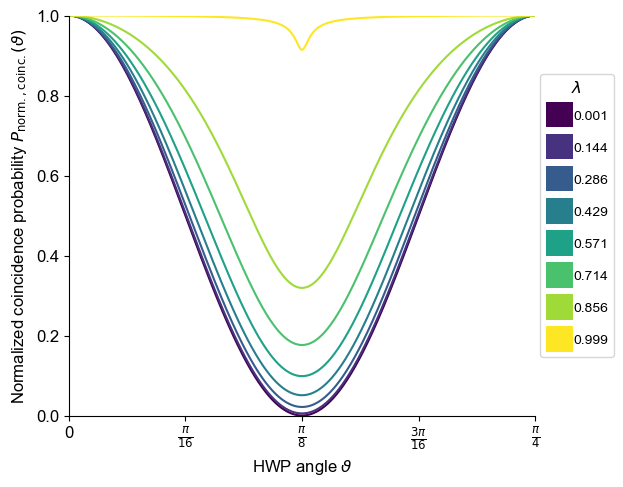
\includegraphics[width=\columnwidth]{cc_probs.png}
    \caption{Probability of measuring coincidences between the output ports of a polarizing beamsplitter at a spcific HWP angle $\vartheta$ for different amounts of squeezing (represented by $\lambda$).}
    \label{fig:tmsv_cc_prob_plot}
\end{figure}
Consequently, the normalized coincidence probability can be expressed as:
\begin{align}
    P_{\text{norm.,coinc.}}(\vartheta)=1-\dfrac{2(1-|\lambda|^2)\left(\dfrac{1}{\sqrt{1-\lambda^2\sin^2(4\vartheta)}}-1\right)}{|\lambda|^2}
\end{align}
Figure \ref{fig:tmsv_cc_prob_plot} depicts this normalized coincidence probability for several values of $\lambda$. As we can see, the higher the amount of squeezing, the lower the depth of the dip at $\vartheta=\pi/8$. This behaviour is due to the higher probability of creating the terms $\ket{n,n}$ (see (\ref{tmsv})) which is connected to $\lambda$.

\section{References}
\renewcommand{\bibsection}{}
\bibliography{sources}% Produces the bibliography via BibTeX.

\appendix
\section{Derivation of the generating function}\label{Derivation:generating_function}
Consider the function $f(y)=(1+y)^z$, which we aim to express as a power series in terms of $y$
\begin{align}
    f(y)=(1+y)^z=\sum_{n=0}^{\infty}a_ny^n,
\end{align}
where $a_n$ are the coefficients we need to determine. 
The Taylor series for a function $f(y)=(1+y)^z$ expanded around $y=0$ is given by
\begin{align}
\label{TaylorExpansion}
    f(y)=\sum_{n=0}^{\infty}\dfrac{f^{(n)}(0)}{n!}y^n,
\end{align}
where $f^{(n)}(y)$ is the $n$-th derivative with respect to $y$ of $f(y)$. These derivatives are
\begin{align}
    f(y)&=(1-y)^z,\\
    f^{(1)}(y)&=z(1+y)^{z-1},\\
    f^{(2)}(y)&=z(z-1)(1+y)^{z-2},\\
    f^{(n)}(y)&=z(z-1)(z-2)...(z-n+1)(1+y)^{z-n}.
\end{align}
At $y=0$ these derivatives become
\begin{align}
    f(0)&=1,\\
    f^{(1)}(0)&=z,\\
    f^{(2)}(0)&=z(z-1),\\
    f^{(n)}(0)&=z(z-1)(z-2)...(z-n+1)\label{derivative:f(y)}.
\end{align}
Substituting (\ref{derivative:f(y)}) into (\ref{TaylorExpansion}) results in
\begin{align}
    f(y)=\sum_{n=0}^{\infty}\dfrac{z(z-1)(z-2)...(z-n+1)}{n!}y^n.
\end{align}
With the generalized binomial coefficient
\begin{align}
    \binom{z}{n}=\dfrac{z(z-1)(z-2)...(z-n+1)}{n!},
\end{align}
we now can get to (\ref{Func:generating_function}) by setting
\begin{align}
    y&=-4x\\
    z&=-\dfrac{1}{2}.
\end{align}
$f(y)=(1+y)^z$ therefore becomes
\begin{align}
\label{Func:generating_func3}
    \dfrac{1}{\sqrt{1-4x}}=\sum_{n=0}^{\infty}\binom{-1/2}{n}(-4x)^n.
\end{align}
Evaluation of the binomial coefficient in this formula gives us
\begin{align}
    \binom{-1/2}{n}&=\dfrac{-\frac{1}{2}(-\frac{1}{2}-1)(-\frac{1}{2}-2)...(-\frac{1}{2}-n+1)}{n!}\\
    \binom{-1/2}{n}&=\dfrac{-\frac{1}{2}(-\frac{3}{2})(-\frac{5}{2})...(-\frac{2n-1}{2})}{n!}\\
    \binom{-1/2}{n}&=\dfrac{(-1)^n(1\cdot3\cdot5\cdot...\cdot(2n-1))}{2^nn!}\label{Eval:binom}
\end{align}
Substituting (\ref{Eval:binom}) back into (\ref{Func:generating_func3}) leaves us with
\begin{align}
    \dfrac{1}{\sqrt{1-4x}}=\sum_{n=0}^{\infty}\dfrac{(-1)^n(1\cdot3\cdot5\cdot...\cdot(2n-1))}{2^nn!}(-4x)^n,
\end{align}
where the factor $(-4x)^n$ can be split into $(-1)^n2^{2n}x^n$, leaving us with
\begin{align}
    \dfrac{1}{\sqrt{1-4x}}&=\sum_{n=0}^{\infty}\dfrac{(1\cdot3\cdot5\cdot...\cdot(2n-1))}{2^nn!}2^{2n}x^n\\
    \dfrac{1}{\sqrt{1-4x}}&=\sum_{n=0}^{\infty}\dfrac{(1\cdot3\cdot5\cdot...\cdot(2n-1))}{n!}2^{n}x^n.\label{Func:generating_func4}
\end{align}
Noticing that $1\cdot3\cdot5\cdot...\cdot(2n-1)$ is the odd part of the double factorial $(2n-1)!!$\cite{Gould2012}, we can use the mathematical identity%\footnote{\url{https://en.wikipedia.org/wiki/Double_factorial}}
\begin{align}
    \label{double_factorial}
    (2n-1)!!=\dfrac{(2n)!}{2^nn!}.
\end{align}
Note that the double factorial $n!!$ is not the same as iteratively applying the factorial, which is written as $(n!)!$ and grows much faster than the double factorial.
Plugging (\ref{double_factorial}) into (\ref{Func:generating_func4}) we get
\begin{align}
    \dfrac{1}{\sqrt{1-4x}}&=\sum_{n=0}^{\infty}\dfrac{(2n)!}{2^nn!n!}2^{n}x^n\\
    \dfrac{1}{\sqrt{1-4x}}&=\sum_{n=0}^{\infty}\dfrac{(2n)!}{(n!)^2}x^n\\
    \dfrac{1}{\sqrt{1-4x}}&=\sum_{n=0}^{\infty}\binom{2n}{n}x^n\label{Func:generating_func_final},
\end{align}
which is the same as in (\ref{Func:generating_function}).
\end{document}

